\chapter{Fine-tuning Enhanced ASR}
\label{chap:fine_tune_enhanced}
In \cref{chap:enhanced_asr}, we proposed the ``Enhanced ASR'' pipeline (see \cref{fig:asr_enhanced_pipeline}) which consists of an \emph{acoustic} model and a \emph{phoneme-to-grapheme translation} model. So far, we used ``clean'' (without any errors) training data to train the translation model. The obvious problem is that the phoneme transcripts produced by the acoustic model in the ASR pipeline will most probably contain errors, to which the translation model is not ready.

In this chapter, we review the fine-tuning of the ASR translation model to errors introduced by the acoustic model.

This chapter is organized as follows: in \cref{feasr:related} we review the related work. \cref{sec:asr_corrupted,sec:asr_corrupted_cs} describe process in which we obtain training data with ``ASR errors''. Finally, \cref{easr:easr} reviews setups for final part of proposer Enhanced ASR pipeline and trains it.

\section{Related Work}
\label{feasr:related}

\citet{hrinchuk2019correction} deal with the correction of errors in ASR by introducing a Transformer post-processing step. 

The authors first train an ensemble of 10 Jasper ASR models on the LibriSpeech dataset. Using these models, they collect ``ASR corrupted'' data (pairs consisting of a transcript from an ASR ensemble model and a correct transcript). To collect more training data, they additionally allow drop-out in the Jasper models during the inference. They also use a Cutout \parcite{devries2017improved} technique that randomly cut rectangles out of the spectrogram. The authors keep pairs with unique ASR transcripts and remove pairs with a word error rate higher than 50 \%. 

Subsequently, they train a Transformer model on this data. The ASR transcripts serve as the source and the original true transcripts as the target. In their best setup, they utilize transfer learning, where they take BERT \citep{devlin2018bert} (notably, a masked language model consisting only of a Transformer encoder) and initialize both encoder and decoder of their Transformer correction model with the BERT's weights.

\section{English ``Corrupted'' Training Data}
\label{sec:asr_corrupted}

In this section, we describe the process in which we gather ``corrupted'' data from the acoustic model. We will use these data later to improve the robustness of the phoneme-to-grapheme translation model.

We design the setup similarly, as described in \cref{feasr:related}. First, we train ten acoustic models. To obtain more data, we additionally store checkpoints during training and keep the last four of them (yielding 40 models). Because of the resource scarcity, we decided to use the QuartzNet architecture instead of Jasper.

Second, we transcribe all available training data using the set of models obtained in the previous step. Subsequently, we pair the ``corrupted'' transcripts with the correct transcripts. Similarly to the \perscite{hrinchuk2019correction}, we apply drop-out and the Cutout during the inference. We obtain a parallel corpus of ``corrupted'' and ``clean'' sentences. We keep only tuples with unique ASR transcripts and remove pairs with PWER higher than 50 \%.

These data will then be used in further training as a source of ``natural'' noise that occurs in speech recognition.

Overview of the setup is pictured in \cref{fig:asr_folds}.

\begin{figure}[t]
	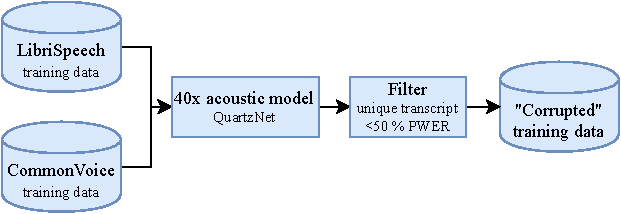
\includegraphics[width=\linewidth]{img/ensemble_diagram}
	\caption{Overview of setup for obtaining ``corrupted'' training data.}
	\label{fig:asr_folds}
\end{figure}

\subsection{Data Preparation}
To train the ensemble of the acoustic models, we use LibriSpeech and Common Voice datasets. We concatenate these two and divide them into ten folds of the same size. We deliberately not shuffle the concatenated dataset prior to splitting it into folds, so that the difference among the trained models is as much as possible (proportion of training data from LibriSpeech and Common Voice will vary more). The models are trained on these folds in a cross-validation manner: $i$-th model skips $i$-th fold during training.

\subsection{Ensemble Training}
We train ten models. Additionally, we store checkpoints every 5000 steps. Instead of bigger Jasper, we choose QuartzNet. Nevertheless, they are similar enough, and we assume they behave likewise. The main reason for our choice are reduced hardware requirements and hence faster convergence. In contrast with the bigger ASR Jasper model that we train on 10 GPUs, each QuertzNet model for data collection is trained only on one GPU. After less than a day of training, the models perform almost as good as the bigger model.

We utilize transfer learning to reduce the training time. For English, the QuartzNet encoders are initialized with checkpoint available at NVIDIA NGC.\footnote{\url{https://ngc.nvidia.com/catalog/models/nvidia:quartznet15x5}} The model was trained on LibriSpeech and Common Voice. As the target vocabulary differs for our setup (phonemes instead of graphemes), we apply the method from chapter \ref{chapter:asr}. The training is divided into the two phases: (1) Decoder adaptation phase: the encoder is initialized with the pre-trained weights and is frozen; the decoder is randomly initialized. Only the decoder is trained. (2) Full training: the encoder is unfrozen and trained together with the decoder. The adaptation phase takes 2000 steps, and full training continues afterward for another 30000 steps.

\subsection{Acoustic Models Performance}
On average, after the first adaptation phase, the word error rate of the most models on LibriSpeech \texttt{dev-clean} dropped under 16 \% (this took approximately 5 hours). One model had WER two times worse than others (33.05 \%), and one did not converge at all. After the full training, which took about 15 hours, the average WER is 5.3 \% with very small variance. Compared with big Jasper, it is only about 1.5 \% points more. Evaluations during the training can be seen in \cref{fig:ensemble_training} and the final results are shown in \cref{tab:eng_folds}.

\begin{figure}[t]
	\includegraphics[width=\linewidth,height=8cm]{img/ensemble}
	\caption{Evaluation on LibriSpeech \texttt{dev-clean} during the training of ten models (using greedy decoding). One epoch takes approximately 24400 steps.}
	\label{fig:ensemble_training}
\end{figure}

\begin{table}[t]
	\centering
	\resizebox{\columnwidth}{!}{
		\begin{tabular}{l|cccccccccc}
			\bf Model & \bf 1 & \bf 2 & \bf 3 & 4 & \bf 5 & \bf 6 & \bf 7 & \bf 8 & \bf 9 & \bf 10  \\
			\hline 
			
			Adapt. phase & 15.17  & 
			15.02  & 
			16.66  & 
			22.15  & 
			15.07  & 
			15.39  & 
			15.24  & 
			17.44  & 
			15.38  & 
			33.05 \\
			Full training &
			5.07  & 
			5.21  & 
			5.16  & 
			4.99  & 
			5.22  & 
			5.34  & 
			5.45  & 
			5.31  & 
			5.30  & 
			5.98
			
		\end{tabular}
	}
	\caption{Results in \% of word error rate (using greedy decoding) on LibriSpeech \texttt{dev-clean} for all trained models.}
	\label{tab:eng_folds}
\end{table}

\subsection{English Corrupted Data Collection}
In order to generate more data, we make checkpoints during training every 5000 steps and keep the last four for every model. This gives us 40 unique models. Additionally, we employ drop-out and Cutout to gain more variability in the collected data.

Concatenated LibriSpeech and Common Voice training data are used as the source for the inference. Using all 40 models, we yield 36M sentence pairs. We keep only the pairs with unique source sentence (i.e., has a unique error) and destroy pairs with PWER over 50 \%. From the 36 million tuples, we get 7M filtered sentence pairs, particularly 3.7M from LibriSpeech and 3.3M from Common Voice.

Distribution of PWER in training and development sets is in histogram~\ref{fig:histogram}. We filter out all pairs with PWER higher than 50~\%. As we can see in the histogram~\ref{fig:histogram}, only 7~\% of all collected training data is left out. We can observe that the distribution of PWER for training data almost copy the distribution of Common Voice \texttt{dev} with training data having slightly more pairs with smaller PWER. On the other hand, LibriSpeech \texttt{dev-clean} has significantly more examples with small PWER.

\begin{table}[t]
	\centering
	\small
	\begin{tabular}{l|ccc}
		\bf Set & \bf AVG WER & \bf Median WER & \bf STD   \\
		\hline 
		Training &  10.24 \% & 2.70 \% & 16.64 \% \\
		LibriSpeech \texttt{dev-clean} &  4.33 \% & 0.0 \% & 8.37 \% \\
		Common Voice \texttt{dev} &  11.98 \% & 0.0 \% & 17.71 \% \\
	\end{tabular}
	\caption{Performance of the 40 ensemble models on the datasets.}
	\label{tab:eng_corrupted_table}
\end{table}

\begin{figure}[t]
	\includegraphics[width=\linewidth,height=8cm]{img/histogram}
	\caption{Distribution of PWER on the collected English ``corrupted'' data and the two development sets.}
	\label{fig:histogram}
\end{figure}









\section{Czech ``Corrupted'' Training Data}
\label{sec:asr_corrupted_cs}
In this section, we reproduce the previously described experiment for the Czech language. Most challenging is to overcome the scarcity of speech data. The Czech speech corpus has approximately 400h. On the other hand, the two English corpora yield together almost 2000h.

\subsection{Task Setup}
We proceed similarly to the setup described in \cref{sec:asr_corrupted}: we split the available data into ``folds''. Each fold then serves as a training corpus for one acoustic model. Unlike for the English, we decided to have only five folds instead of 10 to take the dataset size into account.

The training and collection of corrupted data remain the same.

\subsection{Ensemble Training}
Following the receipt from English, we employ QuartzNet architecture, train all models on one GPU, and follow the same transfer learning technique. We train-off from our best performing, fully trained, Czech ASR model (see \cref{chapter:asr}). Because of the Czech training data scarcity, we train only five folds. For more details regarding the training, see \cref{sec:asr_corrupted}.

\cref{fig:ensemble_training_cs} depicts the performance of the trained acoustic models on the development set during the training.

\subsection{Acoustic Models Performance}
\cref{tab:cs_folds} offers detailed training results for all models. 

We observe a dramatic PWER decline at the beginning (until step 12k), followed by almost no change until the end of the training. We assume there are two reasons for this behavior: (1) data scarcity; (2) contrast in grapheme-to-phoneme correspondence in the Czech and the English language. We assume the latter to have a more significant impact, as the model converged after 7 thousand steps, which is roughly right after seeing all examples once (2000 steps adaptation phase + one epoch of 4775 steps of the full training).

\begin{figure}[h]
	\includegraphics[width=\linewidth,height=8cm]{img/ensemble_cs}
	\caption{Evaluation of the development set during the training of the 5 models (using greedy decoding). One epoch is approximately 4750 steps.}
	\label{fig:ensemble_training_cs}
\end{figure}

\begin{table}[h]
	\centering
	\begin{tabular}{l|cccccccccc}
		\bf Model & \bf 1 & \bf 2 & \bf 3 & 4 & \bf 5  \\
		\hline 
		
		Adapt. phase &
		97.91 &
		17.63 &
		13.53 &
		14.09 &
		13.37 \\
		Full training &
		7.17 &
		7.03 &
		7.14 &
		7.25 &
		7.13 
		
	\end{tabular}
	\caption{Results in \% of PWER (greedy decoding) on the development set for all trained models.}
	\label{tab:cs_folds}
\end{table}

\subsection{Czech Corrupted Data Collection}
In order to generate more data, we make checkpoints during training every 5000 steps and keep the last four for every model. This gives us 20 unique models. Additionally, we employ drop-out and Cutout to gain more variability in the collected data.

We use the training data of the Czech Parliament Hearings dataset as the source for the inference. Using all 20 models, we yield 3.8M sentence pairs. This is almost ten times less than for English. We keep only the pairs with unique source sentences (i.e., has a unique error) and destroy pairs with PWER over 50 \%. Finally, we get two million sentence pairs.

Distribution of PWER in training and dev sets is in histogram~\ref{fig:histogram}. We filter out all pairs with PWER greater than 50~\%. As we can see in the histogram~\ref{fig:histogram}, only 13~\% of all collected training data is removed. We can observe that the collected data contains more recordings with higher PWER than the test set. 

\begin{figure}[t]
	\includegraphics[width=\linewidth,height=8cm]{img/histogram_cs}
	\caption{Distribution of PWER of the collected Czech ``corrupted'' data and the Czech Parliament Hearings test set. Note, we used the test set instead of the development set. PWER of the recordings in the development set does not correspond to the actual sentence-level distribution of PWER. This is because the development set contains 12  further unsegmented recordings each more than 10 minutes long.}
	\label{fig:histogram_cs}
\end{figure}






\section{Fine-Tuning of Enhanced ASR}
In this section, we use the collected ``corrupted'' data to enhance the phoneme-to-grapheme translation models. We experiment with training and fine-tuning using this data. We also examine various transfer learning schemes.

\subsection{Experiment Outline}
We design the fine-tuning experiment similarly to that of \perscite{hrinchuk2019correction} described in \cref{feasr:related}. However, we must consider the differences in our ASR pipeline. Our ASR pipeline consists of an acoustic model transcribing the speech into phonemes, and a phoneme-to-grapheme translation model. On the other hand, the authors have an ASR model to graphemes and a correction model.

In our experiments, we initialize the model weights from SLT tasks. We find the SLT task as a promising starting point for enhancing the ASR transcripts. We base our hopes on the fact that the main task of the encoder in the SLT is to create an abstract representation of the input sentence based on its meaning. This means the encoder must consider the content and semantics of the sentence. Similarly, the decoder must decode the content given by the encoder and is also responsible for creating a meaningful sentence in the target language. This is in contrast with what the Transformer model does when trained as a phoneme-to-grapheme translation model operating within one language. Based on our experience from \cref{chap:enhanced_asr}, we suspect the model remembers rules for rewriting the phonemes to graphemes without considering the context. 

For the English ASR, we experiment with three different setups:

\begin{description}
	\item[Correction Baseline] As a baseline, we train the translation model from scratch. Considering the over-fitting that we observed in \cref{easr:tokenizer} (i.e., when the translation model is trained from scratch solely on corrupted data), we decided to mix (one to one) the corrupted training data with clean phonemized CzEng data.
	
	\item[SLT Transfer] In this setup, we proceed exactly as in the \emph{Correction Baseline}. Additionally, we initialize the Transformer encoder from English to the Czech SLT translation model, and the Transformer decoder is initialized from the Czech to English SLT translation model (see \cref{chap:slt} for more details on SLT).
	
	\item[SLT + BERT Transfer] This setup utilizes a checkpoint from SLT for the encoder and the pretrained BERT for the initialization of the decoder. We do not initialize the encoder as the source of the model are phonemes (thus, we would have to change the tokenizer). We hypothesize this would be a significant change of the task for the pre-trained BERT, and it would diminish the advantage of the pre-training. 
	
	There are several variants of BERT. We decided for \texttt{large-uncased}. We chose the \texttt{large} to match the Transformer encoder (that we initialized from SLT) model dimension (1024).
	
	Additionally, we use only corrupted training data from the LibriSpeech dataset for the fine-tuning. 
\end{description}

For the Czech ASR, we experiment with two setups:

\begin{description}
	\item[Correction Baseline] We train the Czech ASR phoneme-to-grapheme translation model baseline as the English counterpart. We train the model from scratch using a one to one mix of clean phonemized CzEng and corrupted training data (to overcome the over-fitting).
	
	\item[SLT Transfer] We initialize the Transformer model with weights from the SLT task. The encoder is initialized with the encoder from the Czech to English SLT. The decoder is initialized with the decoder from the English to Czech SLT.
	
\end{description}


\subsection{Training/Fine-Tuning}
We train the models on two GPUs with 16 GB VRAM. We set the batch size to 8000 tokens, learning rate to $2 \times 10^{-3}$, and 16000 warm-up steps. The length of the training is set to 6000000, but we manually abort it after the convergence.

All phoneme-to-grapheme models share the same architecture (the Transformer \texttt{big}) except for the \emph{SLT + BERT Transfer}. In this case, the decoder copies the BERT \texttt{large-uncased} architecture (24-layer, 1024-hidden, 16-heads). 

For the \emph{SLT + BERT Transfer}, we tried the same training procedure as for other setups. However, we were unable to obtain any reasonable performance (we got WER of 28\% on LibriSpeech \texttt{dev-other}). We hypothesize this is due to the vast amount of weights that must be randomly initialized in the decoder. The BERT model is essentially a Transformer encoder. Hence it does not have the encoder-decoder attention layer, which must be randomly initialized. During the training of the whole model with many randomly initialized weights, the initially trained weights from the BERT might depart too far from the optimum.

To overcome this issue, we use an analogous adaptation trick as for the training of the acoustic model (see \cref{asr:transfer_phonemes}). We freeze all weights initialized from seed models and train only the randomly initialized weights until the convergence (the criterion was the loss on the validation dataset). This adaptation takes 13500 steps in our case. Subsequently, the training of the whole model continues as in the experiments.

Oversight on the training provides the LibriSpeech \texttt{dev-other} for English, and the Parliament Hearings \texttt{test} for Czech. The overview is in \cref{fig:finetune_en,fig:finetune_cs}. We choose the test set instead of the development set for the Czech as the development set consists of unsegmented long recordings that do not fit into the Transformer model.

\begin{figure}[h]
	\includegraphics[width=\linewidth,height=7cm]{img/finetune_en}
	\caption{Training/fine-tuning of the English phoneme-to-grapheme ASR models. Performance on the LibriSpeech \texttt{dev-other}.}
	\label{fig:finetune_en}
\end{figure}

\begin{figure}[h]
	\includegraphics[width=\linewidth,height=7cm]{img/finetune_cs}
	\caption{Training/fine-tuning of the Czech phoneme-to-grapheme ASR models. Performance on Parliament Hearings \texttt{test}.}
	\label{fig:finetune_cs}
\end{figure}

\subsection{Performance Evaluation}
In this section, we evaluate the performance of the models. For English, we utilize Common Voice \texttt{test} set and LibriSpeech \texttt{test-clean} and \texttt{test-other}. For Czech, we use the test set from Parliament Hearings corpus. The results are in \cref{tab:werstrain,tab:werstrain_cs}.

\paragraph{English} 
From the results in \cref{tab:werstrain}, it is evident that the training/fine-tuning on corrupted data helps. 

Particularly, the \emph{Correction Baseline} and \emph{SLT Transfer} are both trained on data that contains erroneous data from the Common Voice dataset. Both models perform on the Common Voice \texttt{test} very well (3.91 and 3.26 \% WER respectively). On the other hand, the \emph{SLT + BERT Transfer} performs on the Common Voice substantially worse (even worse than the \emph{Clean Baseline}). 

For the LibriSpeech test sets however, we see that the models perform worse when trained on corrupted data containing Common Voice transcripts. The \emph{SLT + BERT Transfer}, which is fine-tuned only on corrupted data from LibriSpeech, performs better than the baseline.

On our \texttt{read-newstest} (for details on the test set see \cref{read-newstest}), the \emph{Correction Baseline} and \emph{SLT Transfer} perform better than the \emph{Clean Baseline}. It seems that both models learned to correct some of the errors. Differently, the \emph{SLT + BERT Transfer}, which was fine-tuned on LibriSpeech corrupted data, performs worse than the \emph{Clean Baseline}. We assume that this is due to the slightly over-fitting of the model to the LibriSpeech corpus.

In the case of \emph{SLT Transfer}, we observe a clear advantage of the initialization from the SLT task over the random initialization (\emph{Correction Baseline}). The training converges rapidly faster, and the final performance is better compared with the random initialization.


\paragraph{Czech}
The results in \cref{tab:werstrain_cs} suggest the same as for the English.

Training using corrupted data enhance the ability of the model to recover from errors introduced by the acoustic model (both models surpass the \emph{Clean Baseline} by more than \XXX{TBD} \% WER). 

Furthermore, it is clear that initializing the models from the SLT task helps in two ways. First, it significantly reduces the training time (by more than 20k global steps --- see \cref{fig:finetune_cs}). Second, it alleviates the final performance of the model.


\begin{table}[t]
	\centering
	\begin{tabular}{l|cccc}
		&\multirow{3}{*}{ \makecell[c]{Common Voice \\ \texttt{test} } } &\multicolumn{2}{c}{LibriSpeech} &\\
		& & \multicolumn{2}{c}{\texttt{test}} & \texttt{read-newstest} \\
		& & {\texttt{clean}} & {\texttt{other}} &\\ \midrule
		Clean Baseline             & 9.72           & 4.87           & 11.67        & 16.38            \\
		%Clean Baseline + LM            & 7.00           & 4.63           & 10.25                   \\
		
		Correction Baseline             & 3.91           & 5.25           & 11.81    & 15.56                \\
		%Correction Baseline + LM            & 4.37           & 5.09           & 10.76                   \\
		
		SLT Transfer     & \textbf{3.26}            & 5.10            & 11.75        & \textbf{15.46}           \\
		%SLT Transfer + LM & 3.97            & 5.00            & 10.63                   \\
		
		SLT + BERT Transfer               & 12.93            & \textbf{4.13}             & \textbf{10.21}  & 19.00       \\      
		%SLT + BERT Transfer + LM & 11.25 & \textbf{4.04}  & \textbf{9.69} \\
	\end{tabular}   
	\caption{Performance of the English ASR phoneme-to-grapheme translation models.}
	\label{tab:werstrain}
\end{table}

\begin{table}[t]
	\centering
	\begin{tabular}{l|cc}
		&  \texttt{test} & \texttt{read-newstest} \\ \midrule
		Clean Baseline             & 9.60       &     33.22         \\
		%Clean Baseline + LM            & 9.35                  \\
		
		Correction Baseline             & 7.44   & 31.94           \\
		%Correction Baseline + LM            & TBD     \\
		
		SLT Transfer     & \textbf{6.54}   & \textbf{29.74}  \\
		%SLT Transfer + LM & 6.92              \\
	\end{tabular}   
	\caption{Performance of the Czech ASR phoneme-to-grapheme translation models on the Czech Parliament Hearings corpus test set.}
	\label{tab:werstrain_cs}
\end{table}


\section{Conclusion and Future Work}
In this chapter, we reviewed a performance-enhancing technique for the proposed ASR pipeline.

First, we gathered ``corrupted'' acoustic data. We trained an ensemble of acoustic models for each language (English and Czech). Consequently, we used these models to gather the corrupted data from speech corpora.

Second, we utilized this data for the training/fine-tuning of the phoneme-to-grapheme translation models from the proposed ASR pipeline. We experimented with different setups. For example, we considered training on mixed ``clean'' and ``corrupted'' data or different transfer learning schemes.

We observed that training-off the checkpoints from the spoken language translation task is the best option. Based on this observation, we suspect that a multi-task training scheme combining SLT and ASR tasks for a language tuple could be promising (i.e., a shared English encoder for English ASR and English-to-Czech SLT decoders, and vice versa).

Further, it is clear that training using ``corrupted'' data helps to reduce the WER. However, the method for obtaining such data is restricted to speech corpora (speech and transcriptions). This is too constraining as speech corpora are generally less available than, for example, free texts (recall, for the training of ASR phoneme-to-grapheme translation we use one side of the CzEng --- phonemized as the source and original as target) which are effortlessly available in almost unlimited amounts. Besides, this scheme is even harder to apply for the SLT, as the speech-to-translation corpora are rare. Finally, the utilization of acoustic models is ``too expensive'' on hardware resources. To overcome these limitations, we see a potential for researching a method that would be able to simulate the errors produced by the acoustic model.


\iffalse 
\begin{figure}[h]
	\centering
	\begin{tikzpicture}[thick, node distance=2.5cm, 
	>=stealth,
	bend angle=45,
	auto,regentonne/.style={cylinder,aspect=0.3,draw,shape border rotate=90}]
	\draw
	node at (0,0)[block,regentonne] (libri) {\shortstack{LibriSpeech\\ \small{training data}}}
	node [block, below right=0.4cm of libri] (ensemble1) {\shortstack{$40 \times$ QuartzNet\\ \small{small models}}}
	node [block,regentonne, below =1.5cm of libri] (common) {\shortstack{Common Voice\\ \small{training data}}}
	
	node at (0,-6) [block,regentonne] (libri_dev) {\shortstack{LibriSpeech\\ \small{dev}}}
	node [block,regentonne, below =0.3cm of libri_dev] (common_dev) {\shortstack{Common Voice\\ \small{dev}}}
	
	node at (5,-7) [block] (jasper) {\shortstack{Jasper\\ \small{big model} \\ \small{from final pipeline}}}
	
	node [block, right=1cm of ensemble1] (filter) {\shortstack{filter\\ \small unique source\\ $<$50\% WER}}
	
	node [block,regentonne,right=1cm of filter] (training) {\shortstack{``corrupted''\\ training data}}
	
	node at (10,-6) [block,regentonne] (libri_dev2) {\shortstack{``corrupted''\\LibriSpeech\\ \small{dev}}}
	node [block,regentonne, below =0.3cm of libri_dev2] (common_dev2) {\shortstack{``corrupted''\\Common Voice\\ \small{dev}}};
	
	\draw[->](libri) -> node {}  (ensemble1);
	\draw[->](common) -> node  {} (ensemble1);
	\draw[->](ensemble1) -> node {}  (filter);
	\draw[->](filter) -> node {}  (training);
	\draw[->](libri_dev) -> node {}  (jasper);
	\draw[->](common_dev) -> node {}  (jasper);
	\draw[->](jasper) -> node {}  (libri_dev2);
	\draw[->](jasper) -> node {}  (common_dev2);
	
	\end{tikzpicture}
	\caption{After training of 10 ``smaller'' QuartzNet models with 4 chechpoints made along the way (hence $40 \times$), training data are transcribed and filtered. Similarly, Development sets are transcribed using ``bigger'' Jasper model that will be in the final ASR pipeline (see \cref{fig:asr_enhanced_pipeline}).}
	\label{fig:asr_folds_}
\end{figure} 
\fi